\documentclass{report}
\usepackage{amsmath}
\usepackage{ngerman}
\usepackage[hidelinks]{hyperref}
\usepackage[numbered]{bookmark}
\usepackage{pgfplots}
\usepgfplotslibrary{fillbetween}
\pgfplotsset{compat=1.18}
\tracinglostchars=2

\title{\textbf{Mathe-Abitur}}
\author{Tim Teichmann}
\date{\today}

\begin{document}
\maketitle
\tableofcontents

\chapter{Funktionsscharen}

\section{Definition}
\begin{flushleft}
    Eine Funktionsschar ist eine Funktion, die auch von anderen Parametern als \(x\) abhängt.
    \begin{align}
        f_k(x)=kx^2
    \end{align}
    Das ist beispielsweise eine quadratische Funktionsschar, die von den Parametern \(x\) und \(k\) abhängt.
\end{flushleft}

\begin{center}
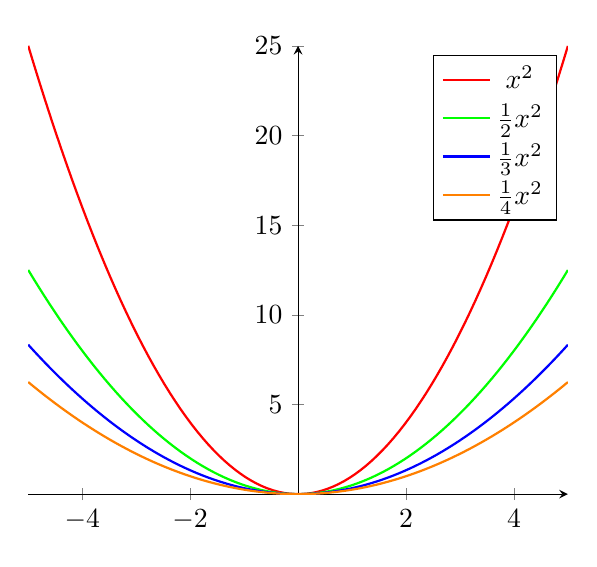
\begin{tikzpicture}
\begin{axis}[
    axis lines=middle,
    samples=100,
    domain=-5:5,
    every axis plot/.append style={thick},
]
\addplot[
    color=red,
]
{x^2};
\addlegendentry{\(x^2\)}

\addplot[
    color=green,
]
{0.5*x^2};
\addlegendentry{\(\frac{1}{2}x^2\)}

\addplot[
    color=blue,
]
{0.3333*x^2};
\addlegendentry{\(\frac{1}{3}x^2\)}

\addplot[
    color=orange,
]
{0.25*x^2};
\addlegendentry{\(\frac{1}{4}x^2\)}

\end{axis}
\end{tikzpicture}
\end{center}

\begin{flushleft}
    Anhand von diesem Beispiel kann man relativ einfach erkennen, dass Funktionen durch Parameter verschiedene Eigenschaften aufweisen können.
\end{flushleft}

\chapter{Integralrechnung}

\section{Stammfunktionen}

\begin{flushleft}
    Stammfunktionen sind Funktionen, die eine Funktion $f$ ergeben, wenn man sie ableitet.
    Also gilt: $F'(x)=f(x)$.

    Allgemein gilt die folgende Regel.
    \begin{align}
        f(x)&=x^n \\
        F(x)&=\frac{x^{n+1}}{n+1}+C, n \in \mathbf{R} - \{-1\}
    \end{align}
    Wenn eine Funktion abgeleitet wird fällt jede Konstante weg, daher gibt es unendlich viele Stammfunktionen, die Konstante wird mit $C$ dargestellt.
\end{flushleft}

\section{Bestimmte Integrale}

\begin{flushleft}
    Bei bestimmten Integralen ist immer klar, welches Intervall gesucht ist.
    Also gilt für ein Integral in dem Intervall $[a;b]$ diese Formel:
    \begin{align}
        \int_{a}^{b} f(x) \ dx = [F(x)]_{a}^{b}
    \end{align}
    Außerdem ist die Integralrechnung keine Flächenberechnung, daher werden oft Absolutbeträge genutzt. Damit wird das Ergebnis eines Integrals immer positiv.
    Die Definition des Absolutbetrags sieht so aus:
    \[
        \mid x \mid =
        \begin{cases}
            x, &\text{wenn } x \geq 0 \\
            -x, &\text{sonst}
        \end{cases}
    \]
\end{flushleft}

\section{Flächen zwischen zwei Funktionen}

\begin{flushleft}
    Um die Fläche zwischen den beiden Funktionen $f$ und $g$ ($f \geq g$) im Intervall $[a;b]$ zu berechnen nutzt man diese Formel:
    \begin{align}
        \int_{a}^{b} [f(x)-g(x)] \ dx
    \end{align}
\end{flushleft}

\section{Mittelwerte von Funktionen}

\begin{flushleft}
    \textbf{diskrete Mittelwerte}: \newline
    Es wird ein Mittelwert aus einer Menge von Zahlen gebildet. \newline
    \begin{align}
        \{1,3&,5,4\} \\
        \frac{1+3+5+4}{4}&=\frac{13}{4}=3.25
    \end{align}
    \newline
    \textbf{kontinuierliche Mittelwerte}: \newline
    Der Mittelwert wird aus Werten einer Funktion bestimmt. \newline
    \begin{align}
        \bar{m}=\frac{1}{b-a}\int_{a}^{b} f(x) \ dx
    \end{align}
\end{flushleft}

\section{Rekonstruktion von Beständen}

\begin{flushleft}
    Bei diesem Aufgabentyp hat man immer eine Funktion (hier: $f$) gegeben, die die momentane Änderungsrate beschreiben soll, also wie stark etwas ansteigt oder fällt.
    Um alle Teilaufgaben vernünftig zu lösen muss man erstmal die Stammfunktion bestimmen:
    \begin{align}
        f(x)&=F'(x) \\
        F(x)&=\int f(x) \ dx
    \end{align}
    Die Konstante $C$, die beim integrieren erscheint sollte in der Aufgabenstellung gegeben sein.
\end{flushleft}

\section{Rotationskörper}

\begin{flushleft}
    Rotationskörper, sind Objekte, die sich bilden wenn eine Funktion um eine Achse rotiert.
    Die Rotationsachse wird auch die Figureachse genannt.
    Um allgemein das Volumen eines Rotationskörpers, der durch die Funktion $f$ beschrieben wird zu bestimmen nutzt man diese Formel:
    \begin{align}
        V=\pi\int_{a}^{b}[f(x)]^2 \ dx
    \end{align}
\end{flushleft}

\section{Uneigentliche Integrale}

\begin{flushleft}
    Uneigentliche Integrale sind bestimmte Integrale mit komplizierteren Integrationsgrenzen.
    Oft wird $-\infty$ oder $+\infty$ in die Integrationsgrenzen eingebaut, es können jedoch auch Integrale mit richtigen Zahlen uneigentlich sein.
\end{flushleft}

\begin{center}
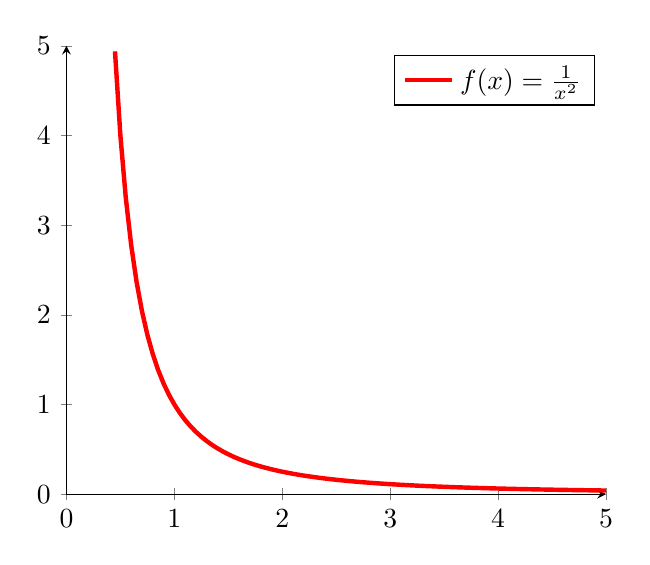
\begin{tikzpicture}
\begin{axis}[
        xmin=0,
        xmax=5,
        ymax=5,
        ymin=0,
        domain=0.05:5,
        samples=100,
        axis y line=left,
        axis x line=bottom,
        restrict y to domain=0:5
        %unbound coords=discard,
    ]
    \addplot[red,ultra thick,name path=A] ({\x},{1/((\x)*(\x))});
    \addlegendentry{\(f(x)=\frac{1}{x^2}\)};
\end{axis}
\end{tikzpicture}
\end{center}

\begin{flushleft}
    Hier sieht man den Plot von $f(x)=\frac{1}{x^2}$.
    Es lässt sich relativ gut erkennen, dass der Wert der Funktion immer größer wird, umso näher man der Y-Achse kommt.
    Entfernt man sich also von der Y-Achse, wird der Wert immer kleiner.
    Mathematisch lässt sich das so ausdrücken:
    \begin{align}
        \lim_{x \to 0} f(x) &= \infty \\
        \lim_{x \to \infty} f(x) &= 0 \\
        \lim_{x \to -\infty} f(x) &= 0
    \end{align}
    Diese Grenzen muss man beachten, wenn man uneigentliche Integrale, wie beispielsweise dieses Integral ausrechnen möchte.
    \begin{align}
        &\int_{1}^{\infty} f(x) \ dx
    \end{align}
    Mit diesem Integral würde man die folgende Fläche berechnen:
\end{flushleft}

\begin{center}
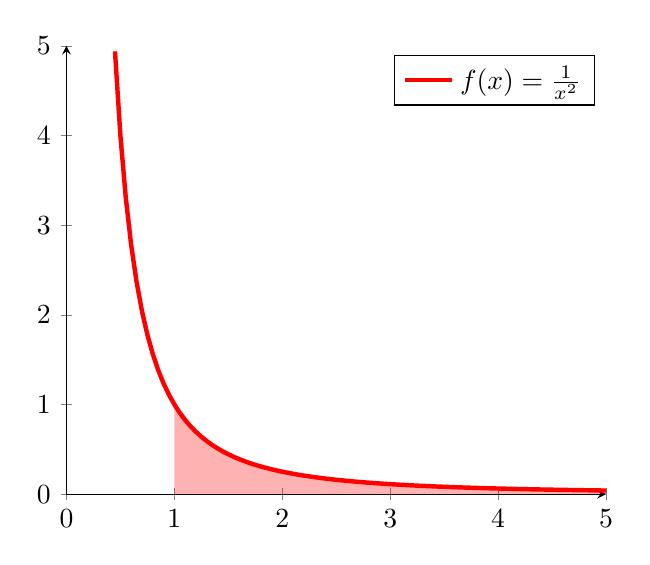
\begin{tikzpicture}
\begin{axis}[
        xmin=0,
        xmax=5,
        ymax=5,
        ymin=0,
        domain=0.05:5,
        samples=100,
        axis y line=left,
        axis x line=bottom,
        restrict y to domain=0:5
        %unbound coords=discard,
    ]
    \addplot[red,ultra thick,name path=A] ({\x},{1/((\x)*(\x))});
    \addlegendentry{\(f(x)=\frac{1}{x^2}\)};
    
    \addplot[draw=none,name path=B] {0};
    \addplot[red,opacity=0.3] fill between[of=A and B,soft clip={domain=1:5}];
\end{axis}
\end{tikzpicture}
\end{center}

\begin{flushleft}
    Wenn man versucht dieses Integral zu berechnen fällt eine Besonderheit auf.
    \begin{align}
        &\int_{1}^{\infty} f(x) \ dx \\
        &\int_{1}^{\infty} \frac{1}{x^2} \ dx \\
        &\int_{1}^{\infty} x^{-2} \ dx \\
        &\left[\frac{x^{-1}}{-1}\right]_{1}^{\infty} \\
        &\left[\frac{-1}{x}\right]_{1}^{\infty}
    \end{align}
    Als obere Grenze kann nicht einfach $\infty$ eingesetzt werden, deshalb suchen wir einen Weg um uns an $\infty$ anzunähern.
    \begin{align}
        &\lim_{b \to \infty} \left[ \frac{-1}{x}\right]_{1}^{b}
    \end{align}
    Jetzt ist es möglich anstatt $\infty$ einfach unsere Variable $b$ einzusetzen und erstmal so weit wie möglich aufzulösen.
    \begin{align}
        &\lim_{b \to \infty} \left[ \frac{-1}{b} - \left(\frac{-1}{1}\right)\right] \\
        &\lim_{b \to \infty} \left( \frac{-1}{b} + 1\right)
    \end{align}
    Nachdem wir so weit wie möglich vereinfacht haben, gucken wir uns jetzt jeden Bestandteil des Ergebnisses an.
    Da unsere Variable $b$ ist, interessieren uns erstmal nur die Terme, in denen $b$ vorkommt.
    $+1$ ist für den Limes irrelevant, da es kein $b$ enthält, $\frac{-1}{b}$ ist jedoch relevant, deshalb müssen wir uns $\frac{-1}{b}$ genauer angucken. \newline
    Dazu müssen wir uns fragen, was passiert, wenn $b$ einen sehr großen Wert annimmt.
    Anhand von ein paar Beispielen kann man das verhalten von $\frac{-1}{b}$ relativ gut verinnerlichen.
    Man kann zur Veranschaulichung einfach ein paar Werte für $b$ einsetzen.
    \begin{align}
        &\frac{-1}{b} \\ 
        \frac{-1}{2} &= -0.5 \\ 
        \frac{-1}{4} &= -0.25 \\ 
        \frac{-1}{8} &= -0.125 \\ 
        \frac{-1}{16} &= -0.0625
    \end{align}
    Wie man relativ gut erkennen kann, geht $\frac{-1}{b}$ immer weiter gegen $0$, desto größer der Wert für $b$ ist.
    Das bedeutet für unsere ursprüngliche Frage, dass dieser Term wegfällt.
    \begin{align}
        \lim_{b \to \infty} &\left( \frac{-1}{b} + 1\right) \\
        &=1 \\
        \int_{1}^{\infty} f(x) \ dx &= 1
    \end{align}
    Nach ein wenig Rechnerei wissen wir also, dass unser uneigentliches Integral, welches eine obere Grenze von $\infty$ hat, nicht den Wert von $\infty$, 
    sondern einen Wert von $1$ hat.
\end{flushleft}

\end{document}
